\documentclass[runningheads]{llncs}

\usepackage[T1]{fontenc}
\usepackage{graphicx}
\usepackage{subcaption}

\begin{document}

\title{TheoremView: A Framework for Extracting Theorem-Like Environments from Raw PDFs}
\titlerunning{TheoremView: Extracting Theorem-Like Environments from Raw PDFs}

\author{Shrey Mishra\inst{1}\orcidID{0009-0004-2357-9593} \and
	Neil Sharma\inst{2}\orcidID{0009-0003-8770-7374} \and
	Antoine Gauquier\inst{1}\orcidID{0009-0005-9573-6364} \and
	Pierre Senellart\inst{1,3}\orcidID{0000-0002-7909-5369}}

\authorrunning{S. Mishra et al.}

\institute{DI ENS, ENS, CNRS, PSL University, Inria, Paris, France \\
	\email{shrey.mishra@ens.psl.eu, antoine.gauquier@ens.psl.eu, pierre@senellart.com}
	\and
	Malaviya National Institute of Technology Jaipur, India \\
	\email{neil.sharma3000@gmail.com}
	\and
	Institut Universitaire de France (IUF)
}

\maketitle

\begin{abstract}
	This paper presents TheoremView, a novel framework for extracting proofs
	and theorems from raw PDF scientific papers without requiring
	\LaTeX~source files. Our approach combines three modalities
	(\textbf{font}, \textbf{text}, and \textbf{vision}) with sequential
	modeling to capture long-term dependencies and layout information. By
	eliminating OCR preprocessing, TheoremView reduces computational overhead
	for real-time applications while providing robust automated theorem
	extraction. Our framework is publicly available at
	\url{https://theoremkb.org/demo}, with a demonstration video at
	\url{https://theoremkb.org/video}.


	\keywords{Theorem extraction \and Multimodal machine learning \and Document analysis \and Natural language processing}
\end{abstract}


\section{Introduction}
\subsection{Motivation for Theorem Extraction}
In contemporary scientific research, articles are primarily published as PDFs, and many
search engines index entire papers instead of specific scientific results. This paper
contributes to TheoremKB~\cite{sdp2024}, a project focused on building a knowledge base of mathematical
results across different fields of science. The objective is to improve the accessibility of
relevant information for researchers, allowing for more effective retrieval and utilization
of scientific knowledge. In particular, TheoremKB aims at streamlining
the retrieval of specific proofs and theorems, allowing quick access to
targeted mathematical results compared to traditional full-text search
engines.

Having such a knowledge base can significantly impact the way researchers
find information~\cite{sdp2024}. Some advantages of this system include:
\begin{enumerate}
	\item \textbf{Enhanced Accessibility}: TheoremKB streamlines the retrieval of specific proofs and theorems, allowing for quick access to targeted mathematical results, in contrast to traditional search engines that index full-text papers.
	\item \textbf{Facilitated Knowledge Discovery}: TheoremKB assists researchers in uncovering connections between disparate mathematical results and their applications, thereby enhancing the exploration of specific results.
	\item \textbf{Identification of Theorem Interdependencies}: TheoremKB helps determine which theorems are used in the proofs of others, which is essential for assessing the impact of errors in foundational results.
	\item \textbf{Support for Automated Reasoning}: TheoremKB provides a foundation for developing AI systems capable of automated theorem proving, promoting innovative approaches to mathematical problem-solving.
\end{enumerate}

\subsection{Prior work on Theorems and Proofs Extraction}

Previous attempts to address this task include the work presented in~\cite{mishra2021towards}, which focused on
initial explorations of extraction from PDFs framed as object detection and text classification problems.
This approach utilized font visuals and text modalities but operated only at the text-line level. Subsequent
research, such as~\cite{mishra2024multimodal}, refined the methodology by incorporating contextual information
surrounding paragraphs and employing multimodal systems to unify the extraction model.
The TheoremView framework offers a user interface to visualize the results extracted by various models in
an end-to-end system that directly takes PDFs as input and displays the extracted results. It is designed
modularly, allowing users to select which model to utilize for extraction, thereby leveraging different
modalities that highlight the strengths and weaknesses of each approach. This flexibility enables users
to run models on low-compute hardware, such as systems without GPU instances, for inference. The primary
objective of this paper is to present an easy-to-use interface that facilitates preprocessing and inference
in a modular manner.

\section{Methodology}
We propose a modular approach to extract raw information from PDFs. We
utilize
\textbf{Grobid}\footnote{\url{https://github.com/kermitt2/grobid}}~\cite{grobid}
and \textbf{pdfalto}\footnote{\url{https://github.com/kermitt2/pdfalto}} to convert
the documents into valid XML formats. The XML data generated by Grobid organizes the content into paragraphs,
while that from pdfalto provides segments content into text lines along with associated font information.
We then employ a merging script to correlate the font information with each paragraph extracted by Grobid.
This process yields a CSV file structured by paragraphs, where each row includes the spatial location of the
paragraph on the page (indicating the page number as well as vertical and horizontal coordinates), the textual content
extracted from Grobid, and the font information used within those
paragraphs. For a schematic diagram of the data pipeline
refer to Fig.~\ref{fig:datapipeline}.

\begin{figure}
	\centering
	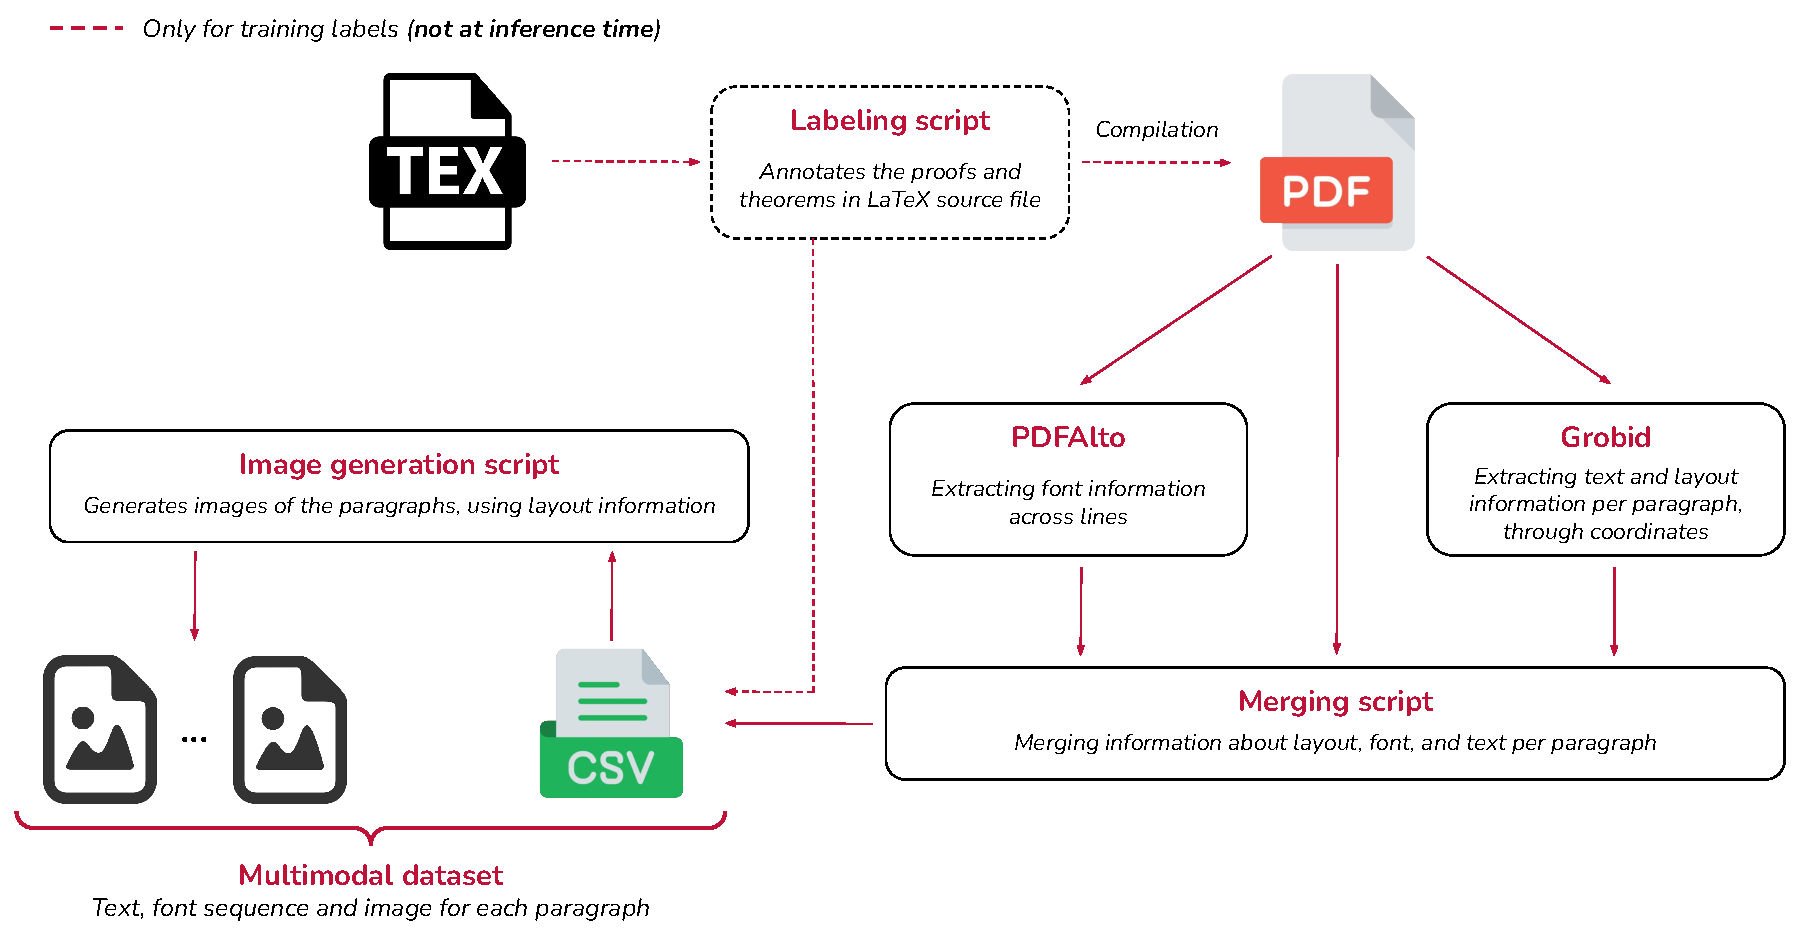
\includegraphics[width=\textwidth]{images/preprocessing.pdf}
	\caption{Data pipeline for extracting and processing information from PDFs}
	\label{fig:datapipeline}
\end{figure}

Once the information is stored in CSV format, we process the font information using an \textbf{LSTM}~\cite{hochreiter1997long} model, where
each font is encoded as a unique token to train the network. Simultaneously, we utilize the bitmap image
rendering of each paragraph to train an \textbf{EfficientNetV2} model
\cite{tan2021efficientnetv2}. Additionally, we employ a \textbf{RoBERTa}-like language model which is pretrained from
scratch \cite{phdthesis},
on a scientific corpus, to make predictions based on the text modality. Subsequently, we
integrate all three trained models into a unified multimodal architecture, freezing the weights of each modality backbone and adding
additional layers to capture intermodality interactions through mechanisms like Gated Multimodal Units
(GMU)~\cite{arevalo2020gated} or cross-modality attention similar to
ViLBERT~\cite{lu2019vilbert} that capture intermodality dependencies.
Refer to Fig.~\ref{fig:generalpipeline} for a summarized view of the
model inference pipeline and to
\cite{mishra2024multimodal,phdthesis} for a detailed presentation of the
architecture.


\begin{figure}
	\centering
	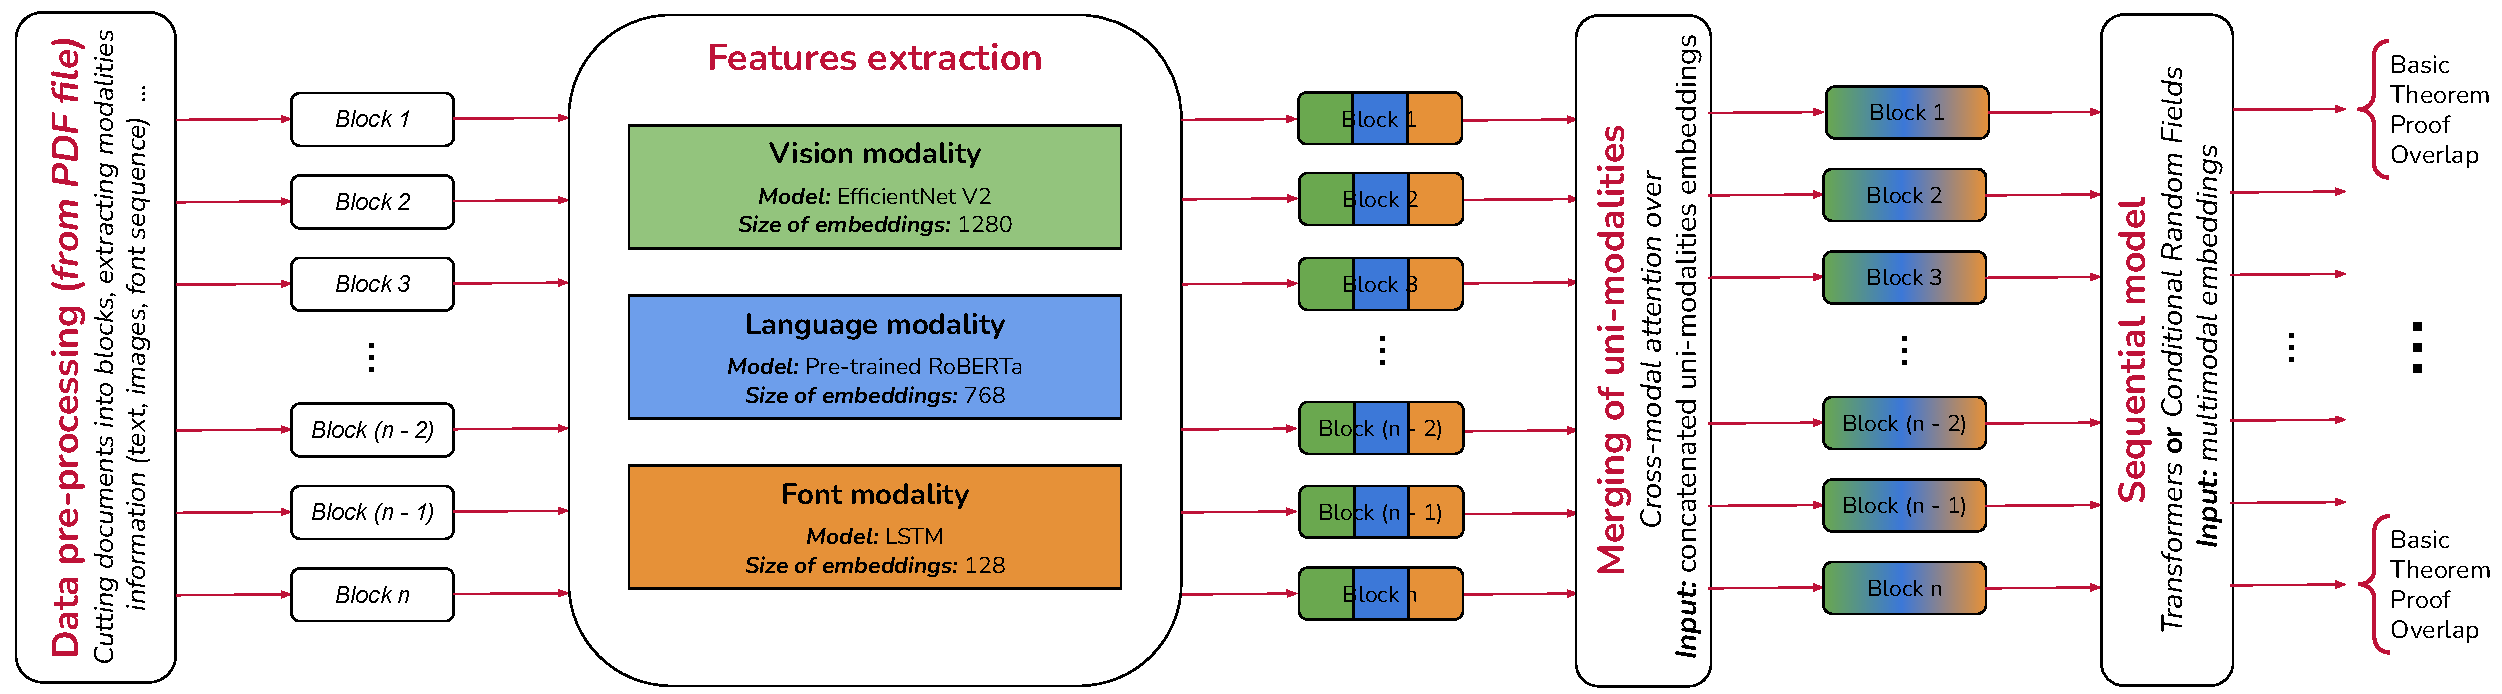
\includegraphics[width=\textwidth]{images/general_pipeline.pdf}
	\caption{Model inference pipeline (adding the sequential paragraph component)}
	\label{fig:generalpipeline}
\end{figure}


With a set of base features extracted from either the unimodal or multimodal approaches, we generate
features for all paragraphs within the PDF. This process incorporates normalized page information,
normalized coordinates of each paragraph, and paragraph embeddings derived from the raw features
just before the softmax layer. To capture sequential information across multiple paragraphs, we train a
Conditional Random Field (CRF)~\cite{CRF2001Lafferty} or Transformer layer on top of the extracted features. The goal is to utilize
relative information to contextualize each paragraph and accurately determine its label. Our model
categorizes paragraphs into four major classes: (1) \textbf{Proof}, (2) \textbf{Theorem-like}, (3) \textbf{Basic} (neither
proof nor theorem), and (4) an \textbf{Overlap} reject class that arises from preprocessing discrepancies.

\section{Demonstration Scenario}

The TheoremView demo interface, built using Streamlit, follows a modular
architecture with distinct functional components. The frontend allows
users to upload PDFs or select from cached samples for metadata
processing using the Grobid and pdfalto tools, with results stored as CSV files. Users can run various ML models (unimodal or multimodal) through a pipeline that calculates processing time, generates bounding boxes, creates cropped images of theorems/proofs, and produces analytical graphs. The system implements efficient caching using pickle files for frequently accessed PDFs and ML model results.

\begin{figure}
	\centering
	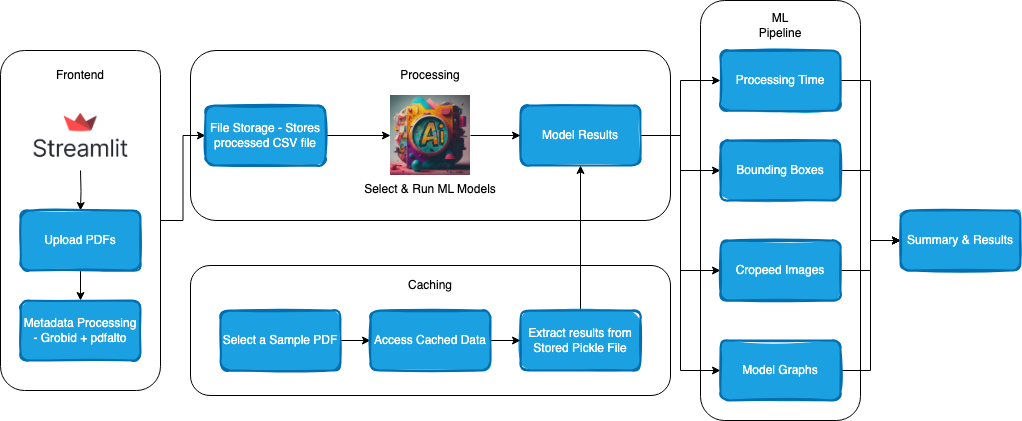
\includegraphics[width=\textwidth]{images/sys-demo-arch.png}
	\caption{System architecture of the various UI components}
	\label{fig:system-arch}
\end{figure}

The UI of the demo is organized into several components (for an overview
see Fig.~\ref{fig:system-arch}), each serving a specific function:

\begin{enumerate}
	\item \textbf{Upload and Process}: Users can upload PDFs or select from cached examples. The system processes PDFs using Grobid and pdfalto, converts pages to bitmap images, and merges XML outputs to generate a preprocessed \texttt{data.csv} file.

	\item \textbf{Predict and Preview}: Users can select unimodal or multimodal base models, with optional sequential processing using CRF, Transformer, or none, offering 12 possible combinations. Results can be previewed or downloaded (see Fig.~\ref{fig:predictions_and_interface}).

	\item \textbf{Summary and Statistics}: Provides a breakdown of inference time for current and cached runs, enabling comparative analysis.
\end{enumerate}

\begin{figure}
	\centering
	\begin{subfigure}[b]{0.48\textwidth}
		\centering
		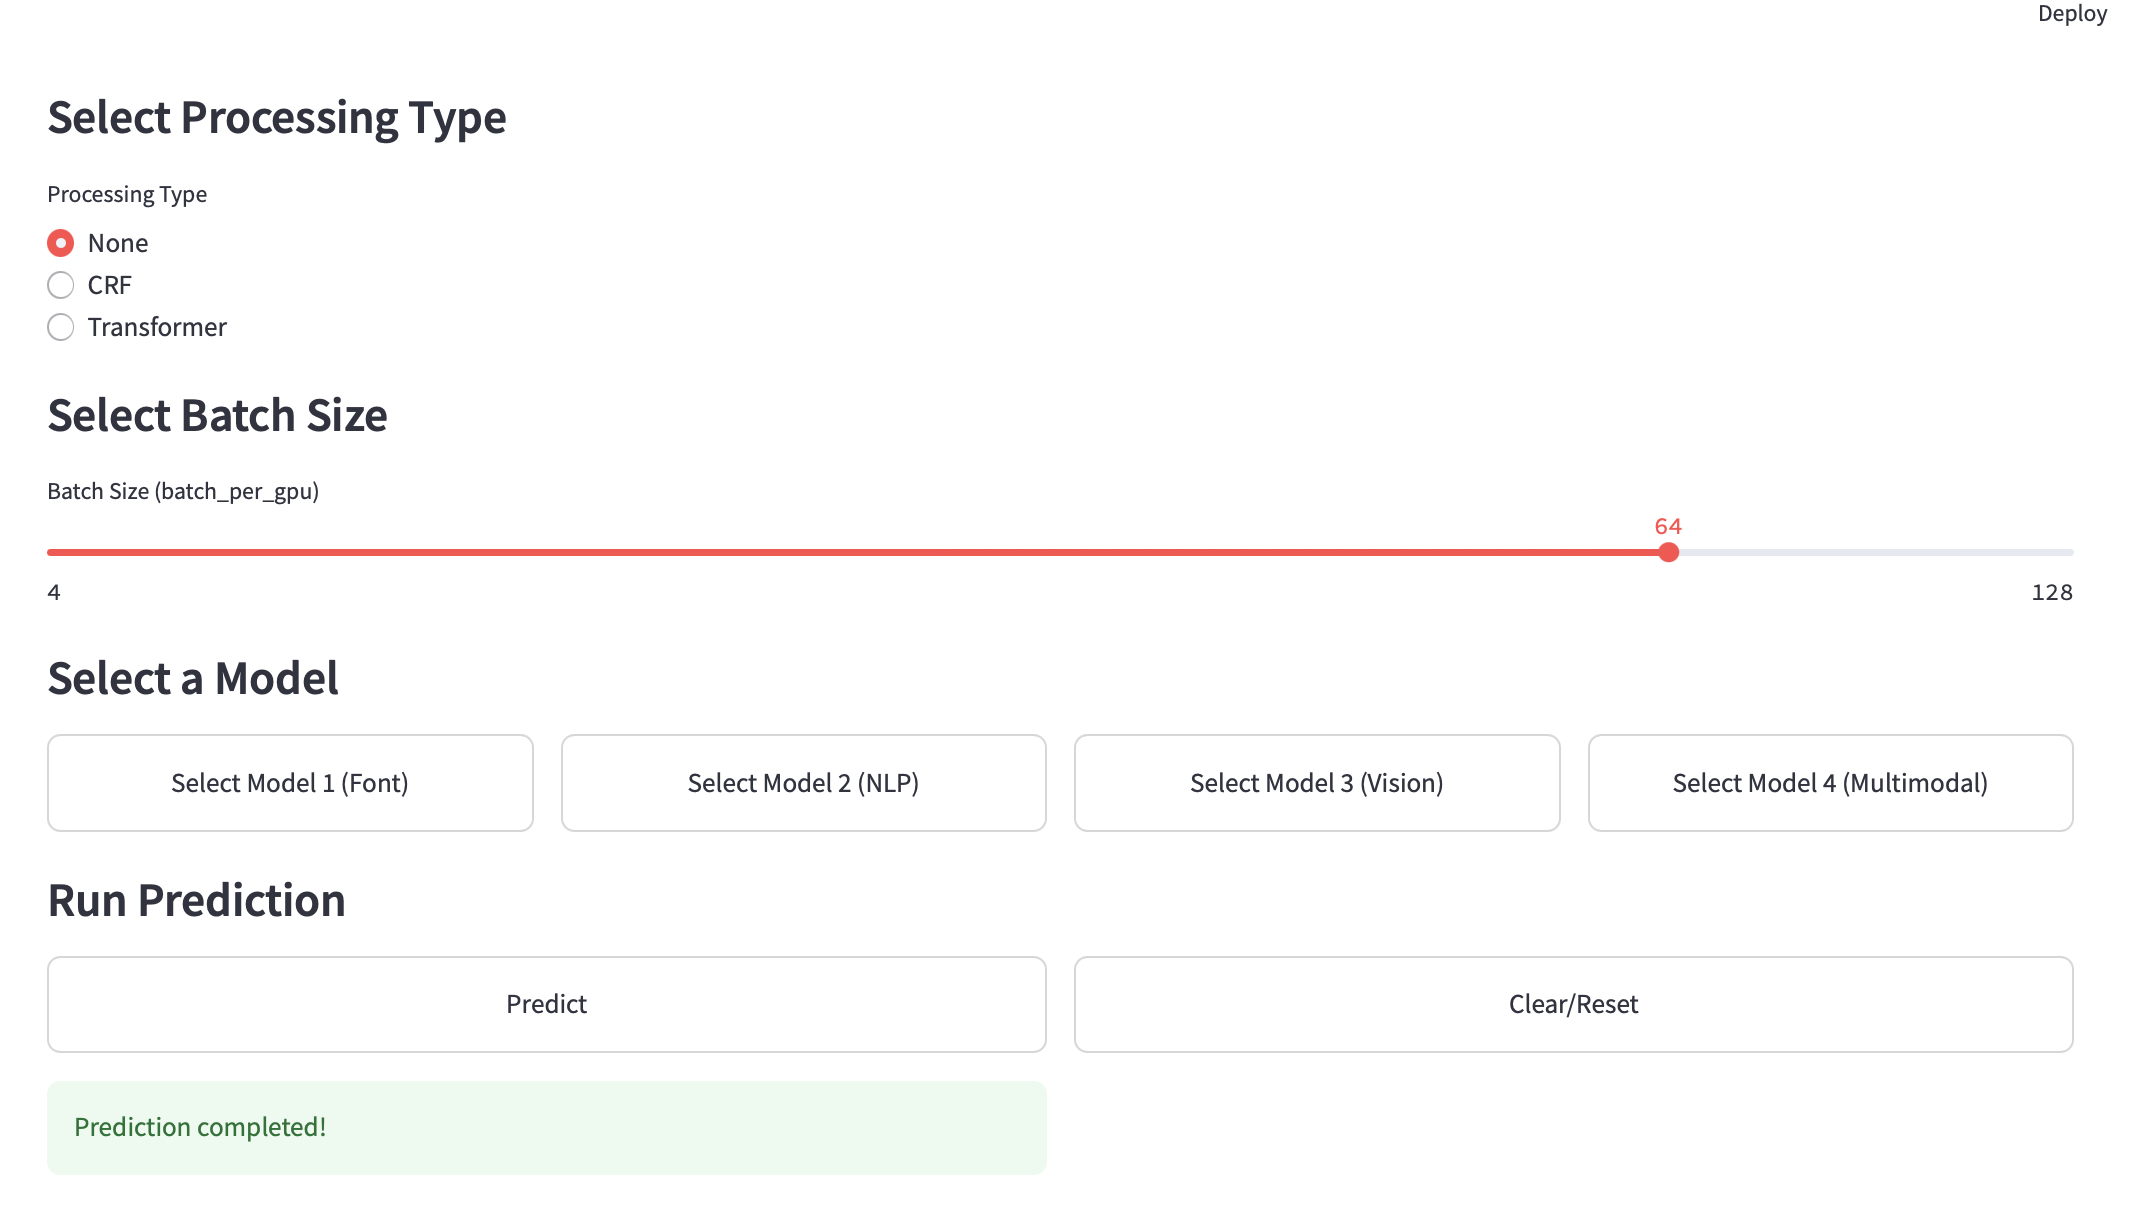
\includegraphics[width=\textwidth]{images/buttons.png}
		\caption{Model selection interface}
	\end{subfigure}
	\hfill
	\begin{subfigure}[b]{0.48\textwidth}
		\centering
		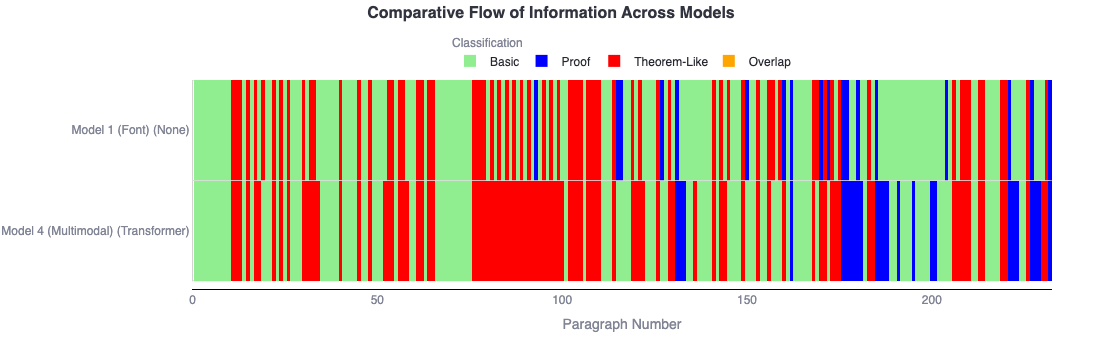
\includegraphics[width=\textwidth]{images/comparitive-v3.png}
		\caption{Flow of information across paragraphs}
	\end{subfigure}

	\vspace{0.5cm}
	\begin{subfigure}[b]{0.48\textwidth}
		\centering
		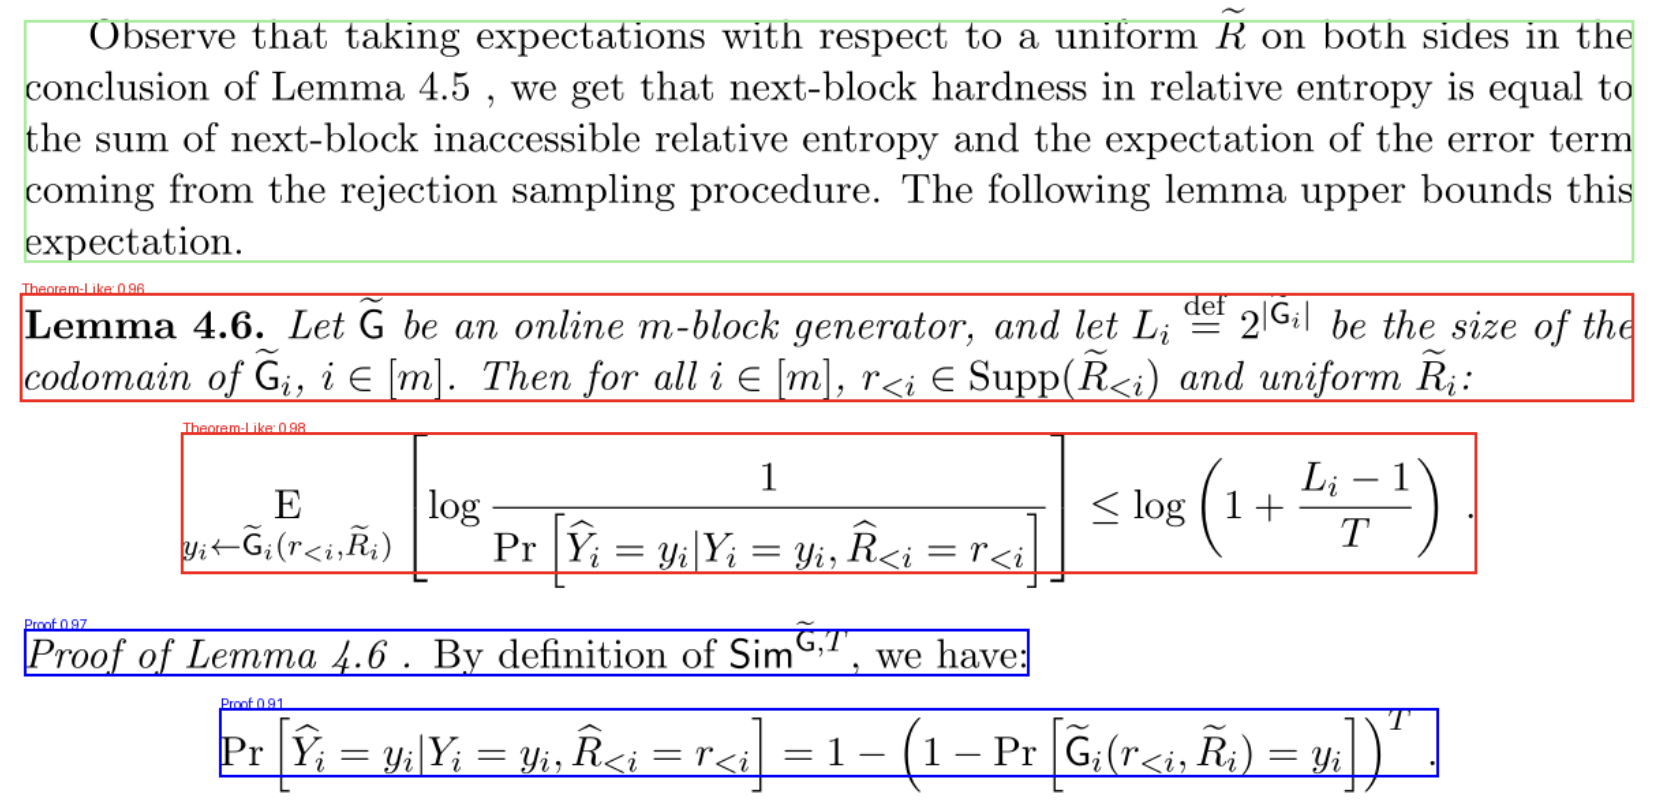
\includegraphics[width=\textwidth]{images/vis_on_pdf.png}
		\caption{PDF rendering with predictions}
	\end{subfigure}
	\hfill
	\begin{subfigure}[b]{0.48\textwidth}
		\centering
		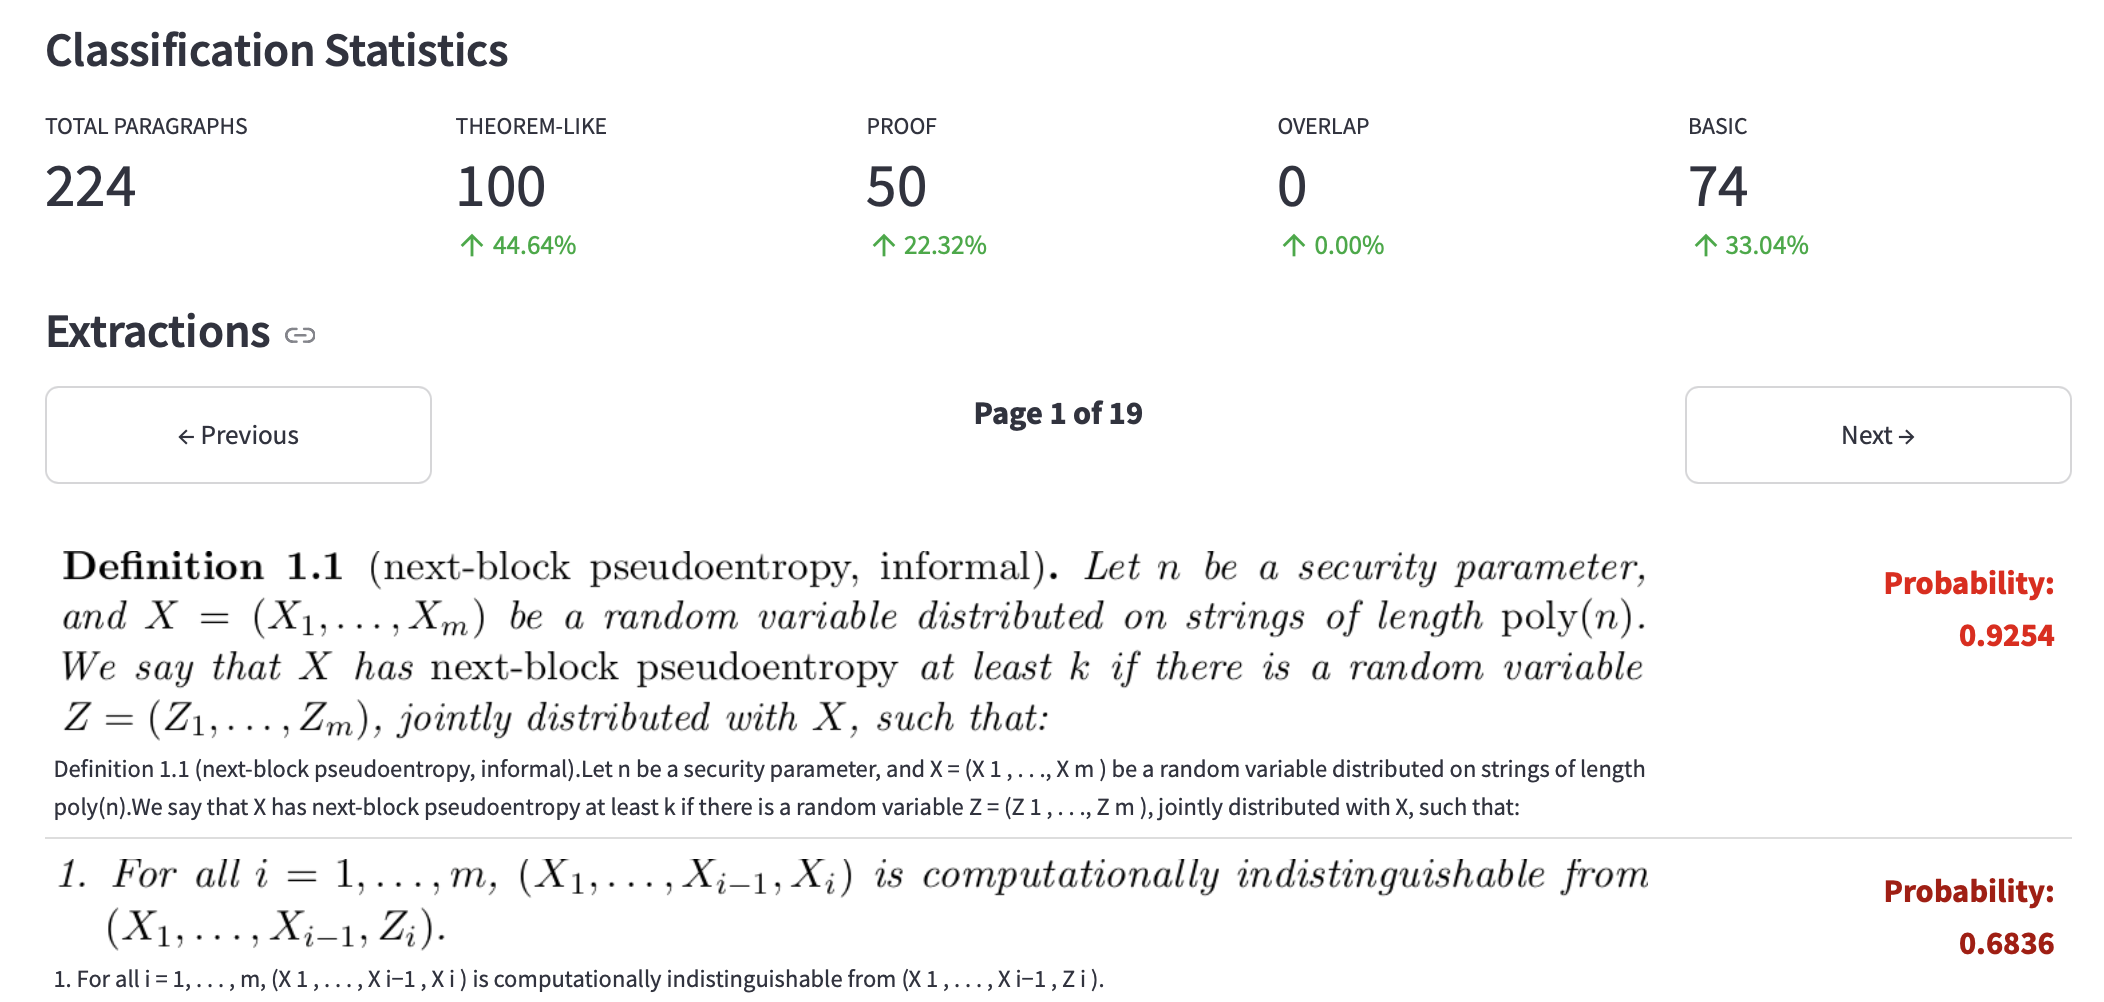
\includegraphics[width=\textwidth]{images/extractions.png}
		\caption{Extraction results}
	\end{subfigure}
	\caption{User interface elements for model selection and predictions}
	\label{fig:predictions_and_interface}
\end{figure}

\begin{credits}
	\subsubsection{\ackname}
	This work was funded in part by the French government under
	management of Agence Nationale de la Recherche as part of the
	“Investissements d’avenir” program, reference ANR-19-P3IA-0001
	(PRAIRIE 3IA Institute). This work was also made possible through
	HPC resources of IDRIS granted under allocation 2020-AD011012097
	made by GENCI (Jean Zay supercomputer).

	\subsubsection{\discintname}
	The authors have no competing interests to declare that are relevant to
	the content of this article.
\end{credits}

\clearpage

\bibliographystyle{splncs04}
\bibliography{bibliography}

\end{document}
